


\tikzset{every picture/.style={line width=0.75pt}} %set default line width to 0.75pt        

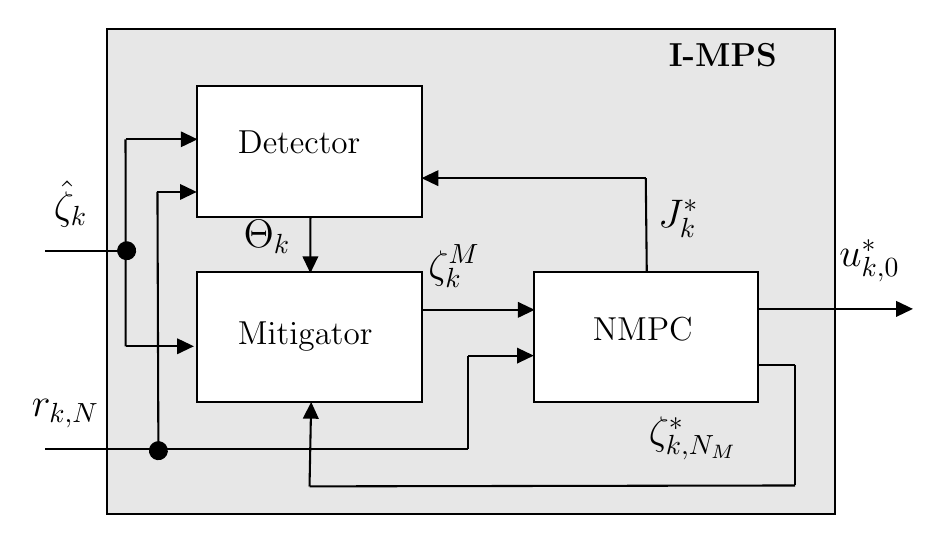
\begin{tikzpicture}[x=0.75pt,y=0.75pt,yscale=-0.9,xscale=0.9]
%uncomment if require: \path (0,300); %set diagram left start at 0, and has height of 300

%Shape: Rectangle [id:dp07321239801052792] 
\draw  [color={rgb, 255:red, 0; green, 0; blue, 0 }  ,draw opacity=1 ][fill={rgb, 255:red, 231; green, 231; blue, 231 }  ,fill opacity=1 ] (121.5,30) -- (511.5,30) -- (511.5,290) -- (121.5,290) -- cycle ;
%Shape: Rectangle [id:dp1563881976892849] 
\draw  [fill={rgb, 255:red, 255; green, 255; blue, 255 }  ,fill opacity=1 ] (170,160) -- (290,160) -- (290,230) -- (170,230) -- cycle ;
%Shape: Rectangle [id:dp978555336465935] 
\draw  [fill={rgb, 255:red, 255; green, 255; blue, 255 }  ,fill opacity=1 ] (170,60.67) -- (290,60.67) -- (290,130.67) -- (170,130.67) -- cycle ;
%Shape: Rectangle [id:dp6438542779108847] 
\draw  [fill={rgb, 255:red, 255; green, 255; blue, 255 }  ,fill opacity=1 ] (350,160) -- (470,160) -- (470,230) -- (350,230) -- cycle ;
%Straight Lines [id:da2661535299648963] 
\draw    (290.5,180.5) -- (347.5,180.5) ;
\draw [shift={(350.5,180.5)}, rotate = 180] [fill={rgb, 255:red, 0; green, 0; blue, 0 }  ][line width=0.08]  [draw opacity=0] (8.93,-4.29) -- (0,0) -- (8.93,4.29) -- cycle    ;
%Straight Lines [id:da9975743928269731] 
\draw    (470,180) -- (550,180) ;
\draw [shift={(553,180)}, rotate = 180] [fill={rgb, 255:red, 0; green, 0; blue, 0 }  ][line width=0.08]  [draw opacity=0] (8.93,-4.29) -- (0,0) -- (8.93,4.29) -- cycle    ;
%Straight Lines [id:da45105295619600305] 
\draw    (410,110) -- (410.55,160.67) ;
%Straight Lines [id:da31332759246635855] 
\draw    (410,110) -- (293,110) ;
\draw [shift={(290,110)}, rotate = 360] [fill={rgb, 255:red, 0; green, 0; blue, 0 }  ][line width=0.08]  [draw opacity=0] (8.93,-4.29) -- (0,0) -- (8.93,4.29) -- cycle    ;
%Straight Lines [id:da6831976187030333] 
\draw    (131.5,89.2) -- (131.55,200) ;
%Straight Lines [id:da5381627981193056] 
\draw    (131.5,89.2) -- (167,89.2) ;
\draw [shift={(170,89.2)}, rotate = 180] [fill={rgb, 255:red, 0; green, 0; blue, 0 }  ][line width=0.08]  [draw opacity=0] (8.93,-4.29) -- (0,0) -- (8.93,4.29) -- cycle    ;
%Straight Lines [id:da9898851017884422] 
\draw    (490,210) -- (490,274.52) ;
%Straight Lines [id:da424908054336965] 
\draw    (470,210) -- (490,210) ;
%Straight Lines [id:da2810640697891009] 
\draw    (230,275) -- (230.82,232.82) ;
\draw [shift={(230.88,229.82)}, rotate = 451.11] [fill={rgb, 255:red, 0; green, 0; blue, 0 }  ][line width=0.08]  [draw opacity=0] (8.93,-4.29) -- (0,0) -- (8.93,4.29) -- cycle    ;
%Straight Lines [id:da4824194165524387] 
\draw    (230,275) -- (490,274.52) ;
%Straight Lines [id:da6654648688677554] 
\draw    (230.5,130.91) -- (230.46,157.85) ;
\draw [shift={(230.45,160.85)}, rotate = 270.09000000000003] [fill={rgb, 255:red, 0; green, 0; blue, 0 }  ][line width=0.08]  [draw opacity=0] (8.93,-4.29) -- (0,0) -- (8.93,4.29) -- cycle    ;
%Shape: Circle [id:dp22585331850262147] 
\draw  [fill={rgb, 255:red, 0; green, 0; blue, 0 }  ,fill opacity=1 ] (127.76,150.09) .. controls (127.07,147.7) and (128.45,145.2) .. (130.84,144.51) .. controls (133.23,143.82) and (135.73,145.2) .. (136.42,147.59) .. controls (137.12,149.98) and (135.74,152.48) .. (133.34,153.17) .. controls (130.95,153.87) and (128.45,152.49) .. (127.76,150.09) -- cycle ;
%Straight Lines [id:da506959418744912] 
\draw    (88.55,148.84) -- (132.09,148.84) ;
%Straight Lines [id:da9298485020674954] 
\draw    (131.55,200) -- (165.05,200) ;
\draw [shift={(168.05,200)}, rotate = 180] [fill={rgb, 255:red, 0; green, 0; blue, 0 }  ][line width=0.08]  [draw opacity=0] (8.93,-4.29) -- (0,0) -- (8.93,4.29) -- cycle    ;
%Straight Lines [id:da32869903555712465] 
\draw    (88.5,255) -- (315,255) ;
%Straight Lines [id:da035880638063171544] 
\draw    (315,205) -- (315,255) ;
%Straight Lines [id:da6563089432200115] 
\draw    (315,205) -- (347,205) ;
\draw [shift={(350,205)}, rotate = 180] [fill={rgb, 255:red, 0; green, 0; blue, 0 }  ][line width=0.08]  [draw opacity=0] (8.93,-4.29) -- (0,0) -- (8.93,4.29) -- cycle    ;
%Shape: Circle [id:dp41684320512129514] 
\draw  [fill={rgb, 255:red, 0; green, 0; blue, 0 }  ,fill opacity=1 ] (144.76,257.14) .. controls (144.07,254.74) and (145.45,252.24) .. (147.84,251.55) .. controls (150.23,250.86) and (152.73,252.24) .. (153.42,254.64) .. controls (154.12,257.03) and (152.74,259.53) .. (150.34,260.22) .. controls (147.95,260.91) and (145.45,259.53) .. (144.76,257.14) -- cycle ;
%Straight Lines [id:da35344859328738143] 
\draw    (148.59,117.39) -- (149.09,255.89) ;
%Straight Lines [id:da8249585929292025] 
\draw    (148.59,117.39) -- (166.59,117.39) ;
\draw [shift={(169.59,117.39)}, rotate = 180] [fill={rgb, 255:red, 0; green, 0; blue, 0 }  ][line width=0.08]  [draw opacity=0] (8.93,-4.29) -- (0,0) -- (8.93,4.29) -- cycle    ;

% Text Node
\draw (420.67,36.17) node [anchor=north west][inner sep=0.75pt]  [font=\large] [align=left] {\textbf{I-MPS}};
% Text Node
\draw (380,183) node [anchor=north west][inner sep=0.75pt]  [font=\large] [align=left] {NMPC};
% Text Node
\draw (190,83) node [anchor=north west][inner sep=0.75pt]  [font=\large] [align=left] {Detector};
% Text Node
\draw (190,185) node [anchor=north west][inner sep=0.75pt]  [font=\large] [align=left] {Mitigator};
% Text Node
\draw (79.67,227) node [anchor=north west][inner sep=0.75pt]  [font=\Large]  {$r_{k,N}$};
% Text Node
\draw (91.5,110) node [anchor=north west][inner sep=0.75pt]  [font=\Large]  {$\hat{\zeta }_{k}$};
% Text Node
\draw (292,144) node [anchor=north west][inner sep=0.75pt]  [font=\Large]  {${\zeta^{M}_{k}}$};
% Text Node
\draw (512,141) node [anchor=north west][inner sep=0.75pt]  [font=\Large]  {$u^{*}_{k,0}$};
% Text Node
\draw (415,120) node [anchor=north west][inner sep=0.75pt]  [font=\Large]  {$J^{*}_{k}$};
% Text Node
\draw (193,131) node [anchor=north west][inner sep=0.75pt]  [font=\Large]  {$\Theta _{k}$};
% Text Node
\draw (410,236.17) node [anchor=north west][inner sep=0.75pt]  [font=\Large]  {$\zeta ^{*}_{k,N_M}$};


\end{tikzpicture}